\documentclass[overlapped,line,final,letterpaper]{res}

%\documentclass[10pt,oneside,a4paper]{article}
\usepackage[spanish]{babel} % Latex en castellano
\usepackage[utf8]{inputenc} % Caracteres con acentos
\usepackage{graphicx}       % Inclusion de graficos
\usepackage{hyperref}

 
%----------------------------------------------------------documento
%----------------------------------------------------------encabezado
\begin{document}

%nombre del personaje
\name{{\Large \bf David Toro Triana}}

\begin{resume}

%-----------------------------------------------datos personales,foto
\vskip 1.0 cm
\vskip 0.5 cm
\begin{minipage}{\linewidth}
	\begin{minipage}{0.5\linewidth} %dirección residencia actual
    		Carrera 15 \# 188-11  \newline %dir
    		Bogotá D.C., Colombia \\ %ciudad
    		313 255 98 64 \\ %cel
    		{\tt dtorot@udistrital.edu.co} \\ %correo
     	{\tt http://opensai.org} \\ %pag-web
	\end{minipage}
	\begin{minipage}{0.5\linewidth}
%		\begin{center}
%			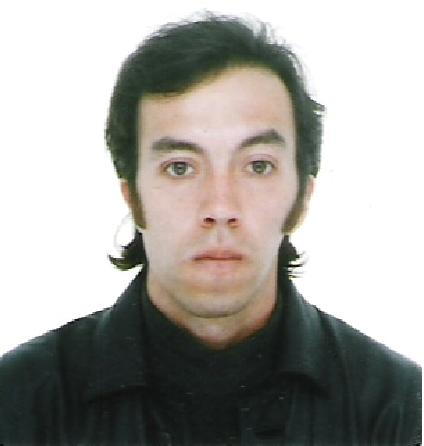
\includegraphics[bb=0 0 100 105, width=30mm,keepaspectratio]{foto.jpeg}
\begin{center}
	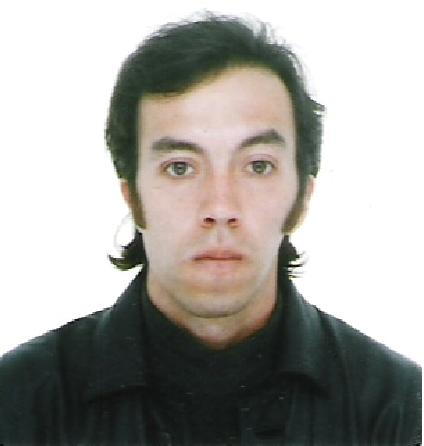
\includegraphics[width=3cm, bb=0 0 305 321]{./foto.jpeg}
	% foto.jpeg: 424x446 pixel, 100dpi, 10.77x11.33 cm, bb=0 0 305 321
\end{center}

%		\end{center}
	\end{minipage}
\end{minipage}


%----------------------------------------------------Perfil
\vspace{0.5cm}
\section{\sc Objetivo}
\vspace{0.5cm}
Crecer personal y profesionalmente usando habilidades para:
\vspace{2mm}
\begin{itemize}
  \item Pensar creativamente y generar soluciones innovadoras
  \item Adquirir, desarrollar y transmitir nuevos conocimientos 
  \item Trabajar en equipo
\end{itemize}

%-----------------------------------------------------Proyectos productivos
% \vspace{1cm}
\vspace{0.5cm}
\section{\sc Proyectos Productivos } %-- twixt \location{} & \begin{position}
\vspace{0.5cm}
% -------------------------------------------
\title{\bf Dirección Ejecutiva
	\newline \em Open Source Academic Initiative.
	\newline {\tt http://opensai.org} 
}
\employer{\em Rep. Legal (S) – \bf Miguel Ángel González Garzón }
\location{\em 320 3614052 – Carrera 46 No 93 - 27 Of. 101 }
\dates{\bf  Enero 2013 – Actualidad }
\begin{position}
Representación legal y dirección de proyectos:
\begin{itemize}
\item Desarrollo de contenidos pedagógicos y acompañamiento al proceso educativo del Programa de Fortalecimiento de Capacidades - Formación en animación digital, 2D, 3D, StopMotion y Efectos Especiales ANIMADELAB (Facultad de Ingeniería, Universidad Nacional de Colombia - 2015)
\item Plataforma de aprendizaje para personas ciegas (Facultad de Ingeniería, Universidad Nacional de Colombia, INCI - 2015)
\item Gestión Plataforma CERI: http://ceri.udistrital.edu.co. El proyecto fue reconocido por el CNA en el 2013, como una de las mejores Buenas Prácticas de Internacionalización - BPI a nivel nacional en el marco de la acreditación de alta calidad: http://www.cna.gov.co/1741/article-320722.html. (Centro de Relaciones Interinstitucionales de la UDFJC,  2013 - 2016)
\item Establecimiento Convenio Marco de Cooperación con la Universidad Nacional de Colombia (Facultad de Ingeniería – Octubre 2014)
\item Establecimiento Convenio Marco de Cooperación con la Universidad Minuto de Dios – \#OpenLAB (Facultad de Ingeniería – Febrero 2017)
\end{itemize}

\end{position}


% -------------------------------------------
\title{\bf Gestión Plataforma Web CERI
	\newline \em Centro de Relaciones Interinstitucionales.
	\newline {\tt http://ceri.udistrital.edu.co} 
}
\employer{\em Director – \bf Dr. Alexis Adamy Ortiz Morales }
\location{\em 323 9300 Ext 1007 – Carrera 7 No 40 - 53 Piso 3 }
\dates{\bf  Julio 2010 – Diciembre 2012 }
\begin{position}
Desarrollo, soporte, mantenimiento, fortalecimiento, construcción de servicios, utilidades, herramientas y contenidos interactivos de La Plataforma Web del Centro de Relaciones Interinstitucionales - CERI. Tomando como base la versión inicialmente creada, e integrando actividades de pertenencia institucional, se modela La Plataforma CERI, que incluía el Directorio de convenios, Membresías, Experiencias, canales sociales oficiales, repositorio de contenidos, documentos y memorias digitales asociadas a las Ferias de Movilidad Académica de la UDFJ.
\end{position} 

% -------------------------------------------
%\title{\bf Diseño e implementación del portal institucional del CERI
%	\newline \em Centro de Relaciones Interinstitucionales.
%	\newline {\tt http://ceri.udistrital.edu.co} 
%}
%\employer{\em Director – \bf Dr. Uriel Coy Verano }
%\location{\em 323 9300 Ext 2005
%	\newline Carrera 7 No 40 - 53 Piso 10 }
%\dates{\bf  Diciembre 2009 – Febrero 2010 }
%\begin{position}
%Responsable de la creación e implementación de lo que en ese momento se concibió como el portal web del Centro de Relaciones Interinstitucionales de la Universidad Distrital Francisco José de Caldas. Esta iniciativa contemplaba la creación de una oficina virtual que apoyara los trámites, procesos y actividades misionales del CERI, integrando una red social especializada en los temas movilidad académica, con el objetivo de beneficiar a la comunidad universitaria cercana a la dependencia. Se logró crear una versión inicial básica pero altamente funcional del modelo planteado.
%\end{position}


% -------------------------------------------
%\title{\bf Voluntario y Asociado
%	\newline \em Open Source Academic Initiative
%	\newline {\tt http://opensai.org} 
%}
%\employer{\em Representante legal – \bf Javier Mora Rincón }
%\location{\em 478 4155 – 300 5182133
%	\newline Carrera 11a No 93a - 62 Of. 303 }
%\dates{\bf  Mayo 2008 – Diciembre 2012 }
%\begin{position}
%Responsable del planteamiento de estrategias, procesos creativos y técnicos. Voluntario capacitador, investigador, desarrollador. En esta etapa, OpenSAI funcionaba como una comunidad dedicada a investigar y transmitir conocimiento técnico en sistemas operativos GNU/Linux [Debian, CentOS, Ubuntu, Gentoo], diseño gráfico [Gimp, inkscape, blender] (entre otras herramientas) a jóvenes talentos, tanto de colegio como universidades. Se realizaban actividades en comunidades, integrando transversalmente temas como la creatividad, Internet, y cultura libre.
%\end{position}

% -------------------------------------------
\title{\bf Dirección de Ingeniería
	\newline \em Tecnologías Xue Ltda.
	\newline {\tt http://xue.com.co} 
}
\employer{\em Representante legal – \bf Verónica González }
\location{\em 256 8089 – 256 4828 – 300 2412225
	\newline Carrera 46 No 93-27 Oficina 101 }
\dates{\bf  Julio 2006 – Febrero 2008 }
\begin{position}
Responsable del diseño, integración-implementación de soluciones de seguridad biométrica y plataformas empresariales basadas en Software Libre, orientadas a la optimización de beneficios para el usuario final y su entorno, utilizando metodologías clásicas de ingeniería de sistemas e ingeniería de software.
\end{position}

%-----------------------------------------------------Proyectos en construcción
\newpage
\opening

% \vspace{1cm}
% \vspace{0.5cm}
%\section{\sc Proyectos en construcción } %-- twixt \location{} & \begin{position}
%\vspace{0.5cm}
%
%\title{\bf Bochica - \em Gestión tecnológica de capital social y cultural}
%\employer{\em Gestor y responsable – \bf David Toro Triana }
%\location{\tt http://bochica.org} 
%\dates{\bf  Enero 2008 – Actualidad }
%\begin{position}
%Colectivo interdisciplinario para la construcción de proyectos autosostenibles de base tecnologica y cultural. Blog personal.
%\end{position}
%
%\title{\bf Mwiska - \em Laboratorio Tecnológico}
%\employer{\em Gestor y responsable – \bf David Toro Triana }
%\location{\tt http://mwiska.com} 
%\dates{\bf  Junio 2008 – Actualidad }
%\begin{position}
%Factoria virtual de investigación y creatividad tecnológica. Intenta ofrecer en un futuro soluciones en ingeniería con el modelo utilizado en \textit{http://guru.com}.
%\end{position}
%
%\title{\bf Otanche - \em Supercomputing Utility}
%\employer{\em Gestor y responsable – \bf David Toro Triana }
%\location{\tt http://otanche.com} 
%\dates{\bf  Enero 2009 – Actualidad }
%\begin{position}
%Diseño e implementación de una plataforma pública de \textit{renderizado}, para las comunidades de artistas que utilizan Blender3D (\textit{http://blender.org}) en su trabajo.
%\end{position}

%-------------------------------------------------------Educación
%\newpage
%\opening
\section{\sc Educación}
\vspace{0.5cm}
Ing., Ingeniería de Sistemas
\newline Proyecto de grado \textit{SISTEMA DE RENDER DISTRIBUIDO TIPO CLUSTER, INTEGRABLE COMO RECURSO A UN ENTORNO DE COMPUTACION GRID}
\newline Universidad Distrital Francisco José de Caldas

\vspace{0.25cm}

%------------------------------------------------------Areas de trabajo
\section{\sc Habilidades y conocimientos especiales}
\vspace{0.5cm}
\begin{itemize}
	\item Configuración y administración de los sistemas operativos GNU/Linux (Debian, Fedora, CentOS), con sus aplicaciones de servicios relacionadas (Apache, MySQL, Nginx, otros)
	\item Adaptación a la medida y administración de entornos web, para gestión de contenido, educación virtual, o comercio electrónico como Moodle, Wordpress, Joomla (otros)
	\item Gestión comunitaria de conocimiento usando MoinMoinWiki o MediaWiki
	\item Programación en lenguajes C/C++, PYTHON
	\item Desarrollo de aplicaciones web con interfaces avanzadas (HTML 5, Bootstrap)
	\item Utilización del framework de desarrollo Django
 	\item Procesos de comunicación, diseño gráfico y construcción de esquemas y presentaciones usando distintas herramientas como Freemind, Inkscape
	\item Sistema de documentación \LaTeX  	
	\item Documentación técnica en inglés

\end{itemize}

%------------------------------------------------------Areas de trabajo
\section{\sc Áreas de interés e investigación}
\vspace{0.5cm}
\begin{itemize}
	\item Gestión de grupos de interés y comunidades virtuales de conocimiento
	\item Procesos de Propiedad Intelectual e Innovación Abierta 
    \item Aplicación social de nuevas tecnologías
    \begin{itemize}
		\item Nuevos modelos educación e inclusión social/digital
	    \item Modelos alternativos de autosuficiencia económica, apropiación cultural, identidad local, sociedad civil y democracia
	    \item Autosuficiencia alimentaria, ecología y sostenibilidad (permacultura)
    \end{itemize}
	\item Computación Gráfica / Computación Científica
    \item Stack’s y pipeline’s IT con sus aplicaciones industriales y académicas de avanzada  (DevOps) 
    \item Buenas prácticas de ingeniería
    \item Seguridad Informática y hacking ético
	
\end{itemize}

\newpage
\opening
\section{\sc Referencias}


Omaira Tovar Ruiz\newline
Instituto Colombiano del Sistema Nervioso Clínica – Monserrat\newline
Calle 134 \# 17 – 71 \newline
2596000 Extensión 6009\newline
{\tt omairatovar@gmail.com} \newline
Profesional en Ciencias de la Información Bibliotecología y Archivista

Cristian Buitrago Ortega\newline
Centro de Gestion de Mercados, Logistica y TIC's\newline
Instructor ADSI - SENA\newline
322 2005004\newline
{\tt cbo@misena.edu.co}\newline
Ingeniero de Sistemas

\vspace{\fill}
\begin{minipage}{1.0\linewidth}
\begin{center}
	
\includegraphics[width=4cm,bb=0 0 598 417]{./firma.jpeg}
	% firma.jpeg: 598x417 pixel, 72dpi, 21.10x14.71 cm, bb=0 0 598 417
\end{center}

\end{minipage}

\vspace{\fill}\ \newline
{\tiny \rm $ $Powered by \LaTeX $ $ }
{\tiny \rm $ $Noviembre 2006$ $ }
{\tiny \rm $ $Nemqueteba Currículum Versión 0.01 $ $ }

\end{resume}
\end{document}
%---------------------------------------------------------------------
%---------------------------------------------------------------------fin documento
